% v2-acmsmall-sample.tex, dated March 6 2012
% This is a sample file for ACM small trim journals
%
% Compilation using 'acmsmall.cls' - version 1.3 (March 2012), Aptara Inc.
% (c) 2010 Association for Computing Machinery (ACM)
%
% Questions/Suggestions/Feedback should be addressed to => "acmtexsupport@aptaracorp.com".
% Users can also go through the FAQs available on the journal's submission webpage.
%
% Steps to compile: latex, bibtex, latex latex
%
% For tracking purposes => this is v1.3 - March 2012

\documentclass[prodmode,acmtecs]{acmsmall} % Aptara syntax
\usepackage{caption}
\usepackage{multicol}
\usepackage{float}
\usepackage{rotating}
\renewcommand{\arraystretch}{1.5}

% Document starts
\begin{document}

% Title portion
\title{Access to Big Data in Bioinformatics}
\author{Brendan Ball\\Andrew van Rooyen}

\acmformat{van Rooyen. Andrew, 2015. Access to Big Data in Bioinformatics}
% At a minimum you need to supply the author names, year and a title.
% IMPORTANT:
% Full first names whenever they are known, surname last, followed by a period.
% In the case of two authors, 'and' is placed between them.
% In the case of three or more authors, the serial comma is used, that is, all author names
% except the last one but including the penultimate author's name are followed by a comma,
% and then 'and' is placed before the final author's name.
% If only first and middle initials are known, then each initial
% is followed by a period and they are separated by a space.
% The remaining information (journal title, volume, article number, date, etc.) is 'auto-generated'.

\maketitle

\section{Project description}
Collaboration between bioinformatics organizations involves shared access to large datasets. This project investigates two avenues for tackling the collaborative analysis of “big data” in bioinformatics: Efficient transport of large datasets across high speed WAN networks and implementation of “community clouds” that host and securely execute code close to the location where data is stored. 

Historically, data has been exchanged using tools and protocols like SSH and FTP, but new protocols, such as GridFTP~\cite{allcock2005globus} and HPN-SSH~\cite{rapier2008high}, offer more efficient use of high speed networks. 

“Community clouds”~\cite{briscoe2009digital} are cloud computing services built on “micro clouds” hosted by collaborating organisations, as opposed to conventional “cloud computing” hosted by cloud vendors (such as Microsoft, Google and Amazon)~\cite{jadeja2012cloud}. Hosting “micro clouds” close to scientific data collections would facilitate scientific collaboration through moving code closer to data, rather than vice versa.

\section{Problem Statement}
The University of Cape Town (UCT) and the University of the Western Cape (UWC) are both part of the South African National Research Network (SANReN). This provides a 10Gb link to other academic institutions in South Africa.
Currently, bioinformatics data in the Western Cape cannot be moved at these speeds, even though the infrastructure theoretically allows it. In practice, the software configuration at the endpoints is the bottleneck. In the scope of this project, the “software configuration” refers to the network protocol, but in practice includes more layers.
This project aims to bring the transfer rate up to the actual capacity of the network by investigating different network protocols.
\\\\
The research question here is: Which network protocol is best for use on a 10Gb/s network, and can it overcome the challenges faced by FTP and SCP?
\\\\
The second part of this project will survey existing cloud computing infrastructures towards their suitability for creating organisation-level micro clouds. The aim is to design and implement a micro cloud solution allowing universities to easily deploy their own micro cloud which can access and be accessed by other connected micro clouds. These connected micro clouds will form a “community cloud”. The micro cloud solution will include implementing a code migration framework which will allow users to easily migrate code between micro clouds, execute that code on the micro cloud which is storing the data and return any results to a specific micro cloud. 
\\\\
The research question for the second part is as follows: “Is it possible to implement a micro cloud platform which provides the convenience of processing bioinformatics data locally, but bypasses the challenges around transferring the data sets?”

\section{Procedures and Methods}
The first part of this project will compare and contrast the performance of GridFTP, HPN-SSH, FTP and SSH for transferring multi-gigabyte datasets. This will be evaluated by comparing throughput, delays, security and authentication features of these protocols and their implementations. Throughput and delays will be measured quantitatively via operating system tools and logging. Other features will be compared by examining literature (whitepapers, definitions) on the protocols themselves.

This will be tested mostly on the local UCT network, and then between UCT and UWC once the nuances of the protocols and their configurations are understood.

For the second part, existing software will be surveyed, and a combination of solutions at various stack levels will be fitted together to form a complete solution. At least two micro clouds will be deployed in order to prototype a community cloud where code can be migrated between micro cloud installations. The community cloud will be evaluated on both its functionality and usability, with more emphasis on functionality. The functionality will be evaluated by testing for the successful processing of given bioinformatics analysis code on example bioinformatics data. Usability testing will be done by doing systematic observation. A limited number of experts will be observed to determine usability using client satisfaction measures.

\section{Ethical, Professional and Legal Issues}
Usually, there would be ethical issues when working with bioinformatics data. However, because this project is only a platform, testing doesn’t rely on having data specific a particular person or group, and it doesn’t have to be recent. Any data we need can be obtained from public sources such as the National Center for Biotechnology Information (NCBI) database.

All experiments for the first section will involve quantitative testing of systems. No ethical issues are raised here. However, access to the UWC network (especially via SANReN) will need to be granted by the appropriate authorities.
There may be user testing involved with the second part, but this will be expert testing with the collaborators of the project. We conclude that no ethical clearance is necessary for this project.

All work will be made publically available under the MIT licence. 

\section{Related Work}
Data sets are a big part of bioinformatics, and have introduced many new challenges with the rise of next generation sequencing. Sequencing technologies like SOLiD provide much higher data output at a cheaper cost~\cite{shendure2008next}, which is good news for research, but troubling for data storage, transfer and access. In fact, the cost of storing a byte has been more expensive than sequencing a base pair since before 2010~\cite{baker2010next}.

This makes it difficult for researchers in different locations to manipulate and run processes on the data, because it will be stored in only one location. These files could be tens of gigabytes in size~\cite{deorowicz2011compression}, depending on context.
\\\\
There has been a lot of work on storing this data. There are a plethora of file formats whose efficiency depends on the kind of data which needs to be stored. Two of the most popular formats are FASTQ, which stores aggregated reads along with the quality of each base pair~\cite{cock2010sanger}, and BAM, the binary, compressed version of the Sequence Alignment Map (SAM) format~\cite{SAMspec}.
\\\\
There are also some proprietary transfer protocols which are widely used in practice. For example, the fasp protocol by the US based company AsperaSoft. Based on UDP, the protocol eliminates the latency issues seen with TCP, and provides bandwidth up to 10 gigabits per second to transfer data~\cite{beloslyudtsev2014aspera}.
\\\\
There has been an explorative push towards cloud solutions from Amazon, Google etc, but there are very significant drawbacks. Because the sequencing happens in labs, researchers need to upload their raw results to the cloud data centres every time they run a new experiment.  This leads back to the original problem, as researchers resort to mailing hard drives~\cite{baker2010next}.

There are also security, privacy and ethical concerns with outsourcing this processing power to other companies, as sequenced DNA data is often highly sensitive information~\cite{marx2013biology}.

Work in this area includes Cloud BioLinux, which is a community driven project focussed on next generation sequencing. It is a toolkit which makes it easy to deploy virtual machines with bioinformatics infrastructure to a cloud platform. It bundles specific packages used in next generation sequence analysis, thereby decreasing configuration time and increasing maintainability Instances of Cloud BioLinux have been tested on the Amazon EC2 cloud platform and on a private Eucalyptus cloud.
\cite{krampis2012cloud}

\section{Possible Future work}
\begin{itemize}
\item Further optimising the data transfer pipeline on different levels of the stack. For example, tuning how data is read from disk to match patterns used by the network layer.
\item Linking user identity to existing databases, and using this as a platform for access control. Users can, for example, have permission to execute code on remote micro clouds if they are trusted.
\item Visualising genomic datasets with software such as Visual Molecular Dynamics (VMD), and linking this to the traditional linear view of the data. Possible advances could involve highlighting areas on a 3D model when a section of the linear data is interacted with. This process would need to run on a cloud and send relevant data back to the user.
\end{itemize}


\section{Anticipated Outcomes}
\begin{itemize}
\item Choice of best transfer protocol for big data in our context of bioinformatics in South Africa.
\item A micro cloud solution providing capability of creating a community cloud.
\end{itemize}

\subsection{Impact}
\begin{itemize}
\item UWC can use their dedicated 10Gbs line
\item Collaboration between universities can increase given the new community cloud platform, particularly in the bioinformatics department.
\end{itemize}

\section{Project Plan}

\begin{sidewaysfigure}[h]
	\fbox{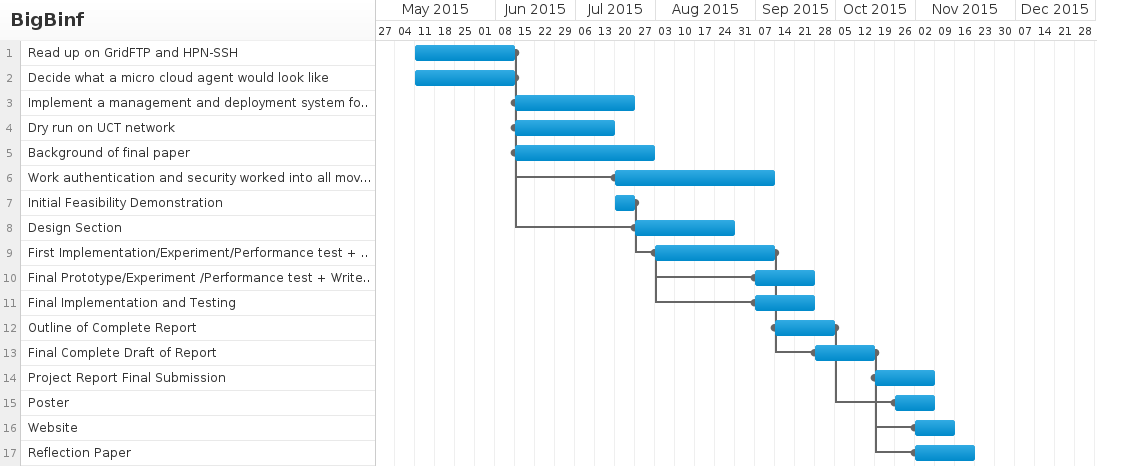
\includegraphics[width=1\textwidth]{img/gantt.png}}
	\caption{Gantt Chart}
	\label{fig:gantt}
\end{sidewaysfigure}

\subsection{Resources Required}
\begin{itemize}
\item Access to servers micro cloud solution 
\item Access to SANReN  for testing transfer protocols
\end{itemize}

\newpage
\subsection{Deliverables}
\vspace*{-40pt}
\begin{multicols}{2}
\begin{itemize}
	\item 24 July - Initial Feasibility Demonstration
	\item 30 July - Background of final paper
	\item 11 September - First Implementation/Experiment/Performance test + Writeup
	\item 21 September - Final Prototype/Experiment /Performance test + Writeup
	\item 25 September - Final Implementation and Testing
	\item 2 October - Outline of Complete Report
	\item 16 October - Final Complete Draft of Report
	\item 2 November - Project Report Final Submission
	\item 2 November - Poster
	\item 9 November - Website
	\item 18 November - Reflection Paper
\end{itemize}
\end{multicols}

\subsection{Milestones}
See see Fig~\ref{fig:gantt} for Gantt chart.
\vspace*{-40pt}
\begin{multicols}{2}
\begin{itemize}
	\item 12 June - Read up on GridFTP and HPN-SSH 
	\item 12 June - Decide what a micro cloud agent would look like
	\item 13 July - Dry run on UCT network  
	\item 20 July - Implement a management and deployment system for the agents
	\item 24 July - Initial Feasibility Demonstration
	\item 30 July - Background of final paper
	\item 28 August - Design Section
	\item 11 September - Authentication and security worked into all moving parts
	\item 11 September - First Implementation/Experiment/Performance test + Writeup
	\item 21 September - Final Prototype/Experiment /Performance test + Writeup
	\item 25 September - Final Implementation and Testing
	\item 2 October - Outline of Complete Report
	\item 16 October - Final Complete Draft of Report
	\item 2 November - Project Report Final Submission
	\item 2 November - Poster
	\item 9 November - Website
	\item 18 November - Reflection Paper
\end{itemize}
\end{multicols}

\subsection{Work Allocation}
\begin{itemize}
\item The first section (comparing transfer protocols) will be completed by van Rooyen. Since this section is anticipated to be shorter than Ball’s, van Rooyen will then work on security and authentication for the cloud platform
\item Ball will do the second section (micro cloud solution)
\end{itemize}

\begin{figure}[H]
	\centering
	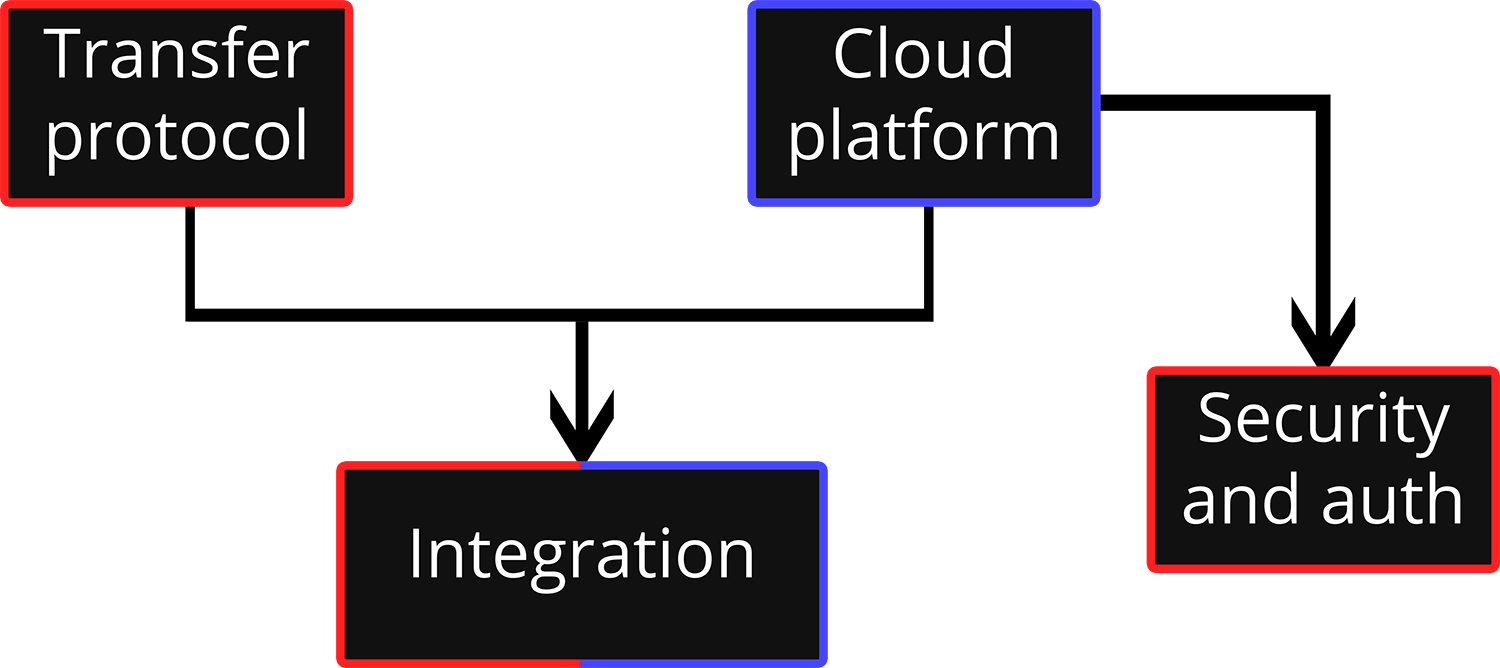
\includegraphics[width=1\textwidth]{img/work_split.png}
	\caption{Work split\\Blue: Ball\\Red: van Rooyen}
	\label{fig:work_split}
\end{figure}

This distribution is not due to any particular skills of van Rooyen or Ball.

\subsection{Risks}
\begin{tabular}{| p{0.5\textwidth} | p{0.5\textwidth} |}
	\hline
	Risk & Mitigation\\
	\hline
	One of the team members is unable to complete his work on time due to unforeseen circumstances
	& The two sections of work are loosely coupled so it won’t prevent the other team member from completing his work\\
	\hline
	Not getting access to key resources
	& Keep open communication with supervisors\\
	\hline
	Project specification is too big, team is unable to complete all tasks on time.
	& Change project specification based on feedback from the presentation\\
	\hline
	Team conflict
	& The project is loosely coupled which should decrease chance of team conflict\\
	\hline
	Failure to integrate project components 
	& Discuss design decisions to account for integration\\
	\hline
\end{tabular}


% Bibliography
\bibliographystyle{ACM-Reference-Format-Journals}
\bibliography{ref}
\end{document}
% End of v2-acmsmall-sample.tex (March 2012) - Gerry Murray, ACM


